\documentclass{article}
\usepackage[utf8]{inputenc}
\usepackage[french]{babel}
\usepackage{hyperref}


\hypersetup{
    colorlinks=fulse,       % false: liens encadrés; true: liens colorés
    linkcolor=red,          % couleur des liens (ou bordures) internes
    citecolor=green,        % couleur des liens (ou bordures) vers bilbio
    filecolor=magenta,      % couleur des liens (ou bordures) vers fichiers
    urlcolor=cyan           % couleur des liens (ou bordures) url
}

\title{ \bf Compte rendu méthode de conception:  Mystic Robot}
\author{ Aubry Nicolas, Leblond Valentin, Mori Baptiste, Chagneux Dimitri}
\date{ \bf Octobre - Novembre 2018}

\usepackage{natbib}
\usepackage{graphicx}
\usepackage{listings}

\begin{document}
\maketitle
\tableofcontents

\vspace{5\baselineskip}

\section{Introduction}
Voici notre jeu, pour la méthode de conception. Nous avons voulu un jeu, avec des règles simples, une approche pour l'utilisateur assez intuitive. Mais en ayant un jeu respectant les différentes règles imposées par l'énoncé.

\section{Le jeu }

\subsection{Les règles du jeu : }

À chaque tour de jeu, les joueurs jouent l'un après l'autre selon un ordre initialement défini, ou selon un ordre tiré aléatoirement à chaque tour.

\vspace{1\baselineskip}

\subsubsection{Une action possible est:}

\vspace{1\baselineskip}

\begin{itemize}
    \item  Déplacement d'une case (4 directions possibles seulement).
    \item  Dépôt d'une mine ou d'une bombe sur l'une des 8 cases voisines.
    \item  Utilisation d'un tir horizontal ou d'un tir vertical.
    \item  Déclenchement du bouclier, qui protège des tirs et bombes lors du prochain tour.
    \item  Ne rien faire pour économiser son énergie.
\end{itemize}

\vspace{1\baselineskip}

\subsubsection{La grille :}

La grille peut contenir, lors de sa création, des murs (cases non-utilisables par les combattants et infranchissables par les tirs), et des pastilles d'énergie que les combattants peuvent récupérer en se plaçant dessus.

\vspace{1\baselineskip}

\subsubsection{Les bombes, mines, tirs et shield :}

\vspace{1\baselineskip}

\begin{itemize}
    \item Une mine explose lorsqu'un combattant se place sur la case qu'elle occupe.
    \item Une bombe explose au bout d'un certain délai t (compte à rebours en nombre de tours de jeu),
	et impacte les combattants se trouvant sur l'une des 8 cases voisines, ou , comme une mine,	si l'on se place dessus.
	\item Les bombes et les mines peuvent avoir deux types de visibilité: visible de tous les combattants, ou visible seulement du combattant qui l'a déposée.
	\item Un tir horizontal impacte les combattants se trouvant sur la même ligne horizontale, à un nombre de cases inférieur à la distance (portée limitée). Idem pour un tir vertical (i.e sur la même colonne).
	\item Une explosion ou un tir impactant un combattant fait baisser son énergie d'une certaine valeur qui fera partie des paramètres du jeu.
	\item Un déplacement et l'utilisation du bouclier ont eux aussi leurs coûts respectifs.
    \item Un combattant perd le jeu lorsque son énergie est négative ou nulle. Il disparaît alors du jeu.
    \item Le gagnant est le dernier survivant.
\end{itemize}

\vspace{1\baselineskip}

\section{Diagramme UML du jeu :}

\subsection{Le diagramme :}

\vspace{3\baselineskip}


\begin{figure}[ht]
   \caption{\label Voici notre Diagramme UML}
   \vspace{0.5\baselineskip}
   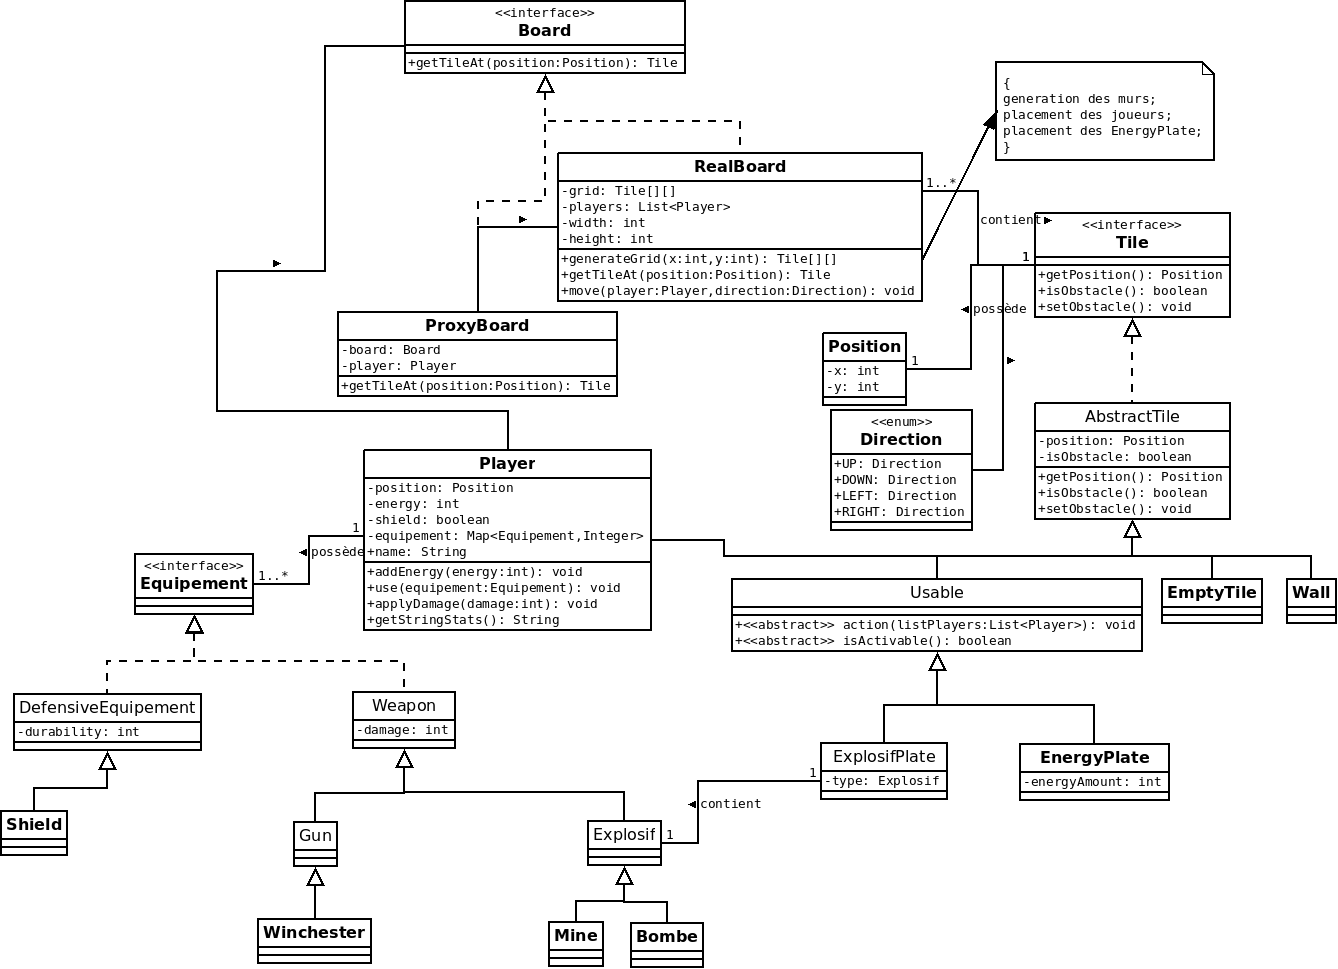
\includegraphics[scale=0.25]{DiagrammeUML.png}
\end{figure}




\vspace{1\baselineskip}

\subsection{Explications :}

Nous avons voulu, un diagramme simple, mais en même temps assez complet afin de pouvoir s'y retrouver facilement et que toutes les personnes du groupe puissent le comprendre assez aisément. Ensuite, nous avons voulu le maximiser un maximum, c'est-à-dire éviter les redondances, les classes inutiles et la répétition de code inutile.

\vspace{0.3\baselineskip}

Donc après plusieurs relectures du diagramme et du code, nous avons pu ainsi enlever des parties du code qui devenaient à nos yeux inutiles.

\vspace{1\baselineskip}

\section{Les patterns et modèles utilisés:}

\subsection{Le pattern Strategy:}


Le pattern Strategy est un pattern qui permet d'externaliser le contenu de certaines méthodes pour pouvoir modifier les comportements soit dynamiquement, soit en utilisant de nouvelles implémentations.


\subsection{Le pattern Factory:}

Le pattern Factory permet de générer dynamiquement des types d'objets.

Voici un exemple de code dans lequel nous utilisons le pattern Factory:


\lstinputlisting[language=Java, firstline=2, lastline=7]{Winchester.java}

\vspace{0.3\baselineskip}

Dans notre projet, on se sert du pattern afin de créer des objets Player qui ont des caractéristiques prédéfinies (énergie, stuff, rôle, etc.).
On l'utilise dans la classe RobotFactory, c'est grâce à cela que l'on arrive à dire si on a des joueurs de types sniper, tank ou autres.

\vspace{1\baselineskip}




\vspace{1\baselineskip}

\subsection{Le pattern Proxy:}

Le pattern Proxy permet de servir d'intermédiaire entre l'objet à contrôler et celui qui veut y accéder.

\vspace{1\baselineskip}

Dans notre jeu, nous avons implémenté le pattern Proxy, afin de permettre aux différents joueurs de ne pas voir les mines disposées par les ennemis. Mais de voir seulement les mines ou bombes que le joueur a lui-même poser.

\vspace{1\baselineskip}

Voici un exemple de ce que cela peut donner graphiquement (cf: Figure 2) :

\begin{figure}[ht]
   \caption{\label Exemple d'utilisation du pattern Proxy :}
   \vspace{0.5\baselineskip}
   \includegraphics[scale=0.60]{GUI.PNG}
\end{figure}


\subsection{Le pattern Decorator:}

Le pattern Décorator permet d'éviter la redondance et l'explosion du nombre de classes. Donc on créer un objet B qui se fait passer pour un objet A en enrichissant ses fonctionnalités.


\subsection{ \bf Le modèle MVC:}

\vspace{1.5\baselineskip}

\subsubsection{Le Modèle :}


\vspace{1\baselineskip}

Le Modèle : Notre modèle est composé du package game, qui contient toutes nos classes gérant le modèle.

\vspace{1\baselineskip}

\subsubsection{La Vue :}

\vspace{1\baselineskip}

La Vue : La vue, elle nous sert à afficher graphiquement notre jeu. Nous utilisons les JFrames ainsi que les JPanel. Notre vue est composée du package gui, qui contient toutes les classes permettant de générer graphiquement nos différentes interfaces graphiques.

\vspace{1\baselineskip}

\subsubsection{Le Contrôleur :}

\vspace{1\baselineskip}

Le Contrôleur : Le contrôleur est aussi composé du package gui.

\vspace{1\baselineskip}

\section{Test du jeu :}

Pour les tests de notre jeu, nous vous mettons des images afin de voir le résultat sur différentes situations. Par exemple la pose d'une bombe, la mort d'un joueur, l'explosion d'une bombe, etc.


\section{Conclusion}

La matière méthode de conception, nous a permis de mieux comprendre certains aspects de programmation ( Par exemple l'utilisation des différents patterns vus durant les CM et TP. ). De plus, la répartition des taches a été un des piliers centraux, concernant la mise en place du jeu.

\vspace{0.5\baselineskip}

Le plus long dans la gestion de ce projet a été de mettre en place les différents Pattterns comment les implémenter, ou les mettre, lesquels nous sont utiles et lesquels nous seront inutiles. Le plus long a été la mise en place du jeu en façon "console". Car nous avons d'abord dû tout implémenter avant de commencer à vraiment réaliser l'interface graphique de notre jeu.

\vspace{0.5\baselineskip}

Ce projet nous aura permis de mieux comprendre les différentes façons de concevoir la mise en place d'un projet à rendre, du papier à la version finale. Comment bien commencer et les bonnes façons d'y parvenir.


\section{Références}

\subsection{Références bibliographiques :}

\bibliographystyle{plain}
\bibliography{references}

\vspace{1\baselineskip}

\bf Référence aux différents CM et TP de Yann Mathet.

\vspace{0.5\baselineskip}

\url{https://mathet.users.greyc.fr/}

\vspace{0.3\baselineskip}

\url{https://ecampus.unicaen.fr/course/view.php?id=15145}

\vspace{0.5\baselineskip}

\subsection{Références externes :}

\vspace{1\baselineskip}

\bf Référence aussi à différentes documentations présentes en ligne :

\vspace{0.3\baselineskip}

\bf Concernant la mise en page latex:

\vspace{0.5\baselineskip}

\url{http://www.xm1math.net/doculatex/url.html}

\vspace{0.3\baselineskip}

\url{https://urlz.fr/8eFS}

\vspace{0.3\baselineskip}

\url{https://docs.oracle.com/javase/7/docs/index.html}

\vspace{0.3\baselineskip}

\url{https://stackoverflow.com/questions/50439945/strategy-pattern-java}

\vspace{0.3\baselineskip}

\end{document}
